% Created 2024-07-08 Mon 22:16
% Intended LaTeX compiler: pdflatex
\documentclass[11pt]{article}
\usepackage[utf8]{inputenc}
\usepackage[T1]{fontenc}
\usepackage{caladea}
\usepackage{graphicx}
\usepackage{longtable}
\usepackage{wrapfig}
\usepackage{rotating}
\usepackage[normalem]{ulem}
\usepackage{amsmath}
\usepackage{amssymb}
\usepackage{capt-of}
\usepackage{hyperref}
\usepackage{fancyhdr}
\usepackage{tikz}

\title{
  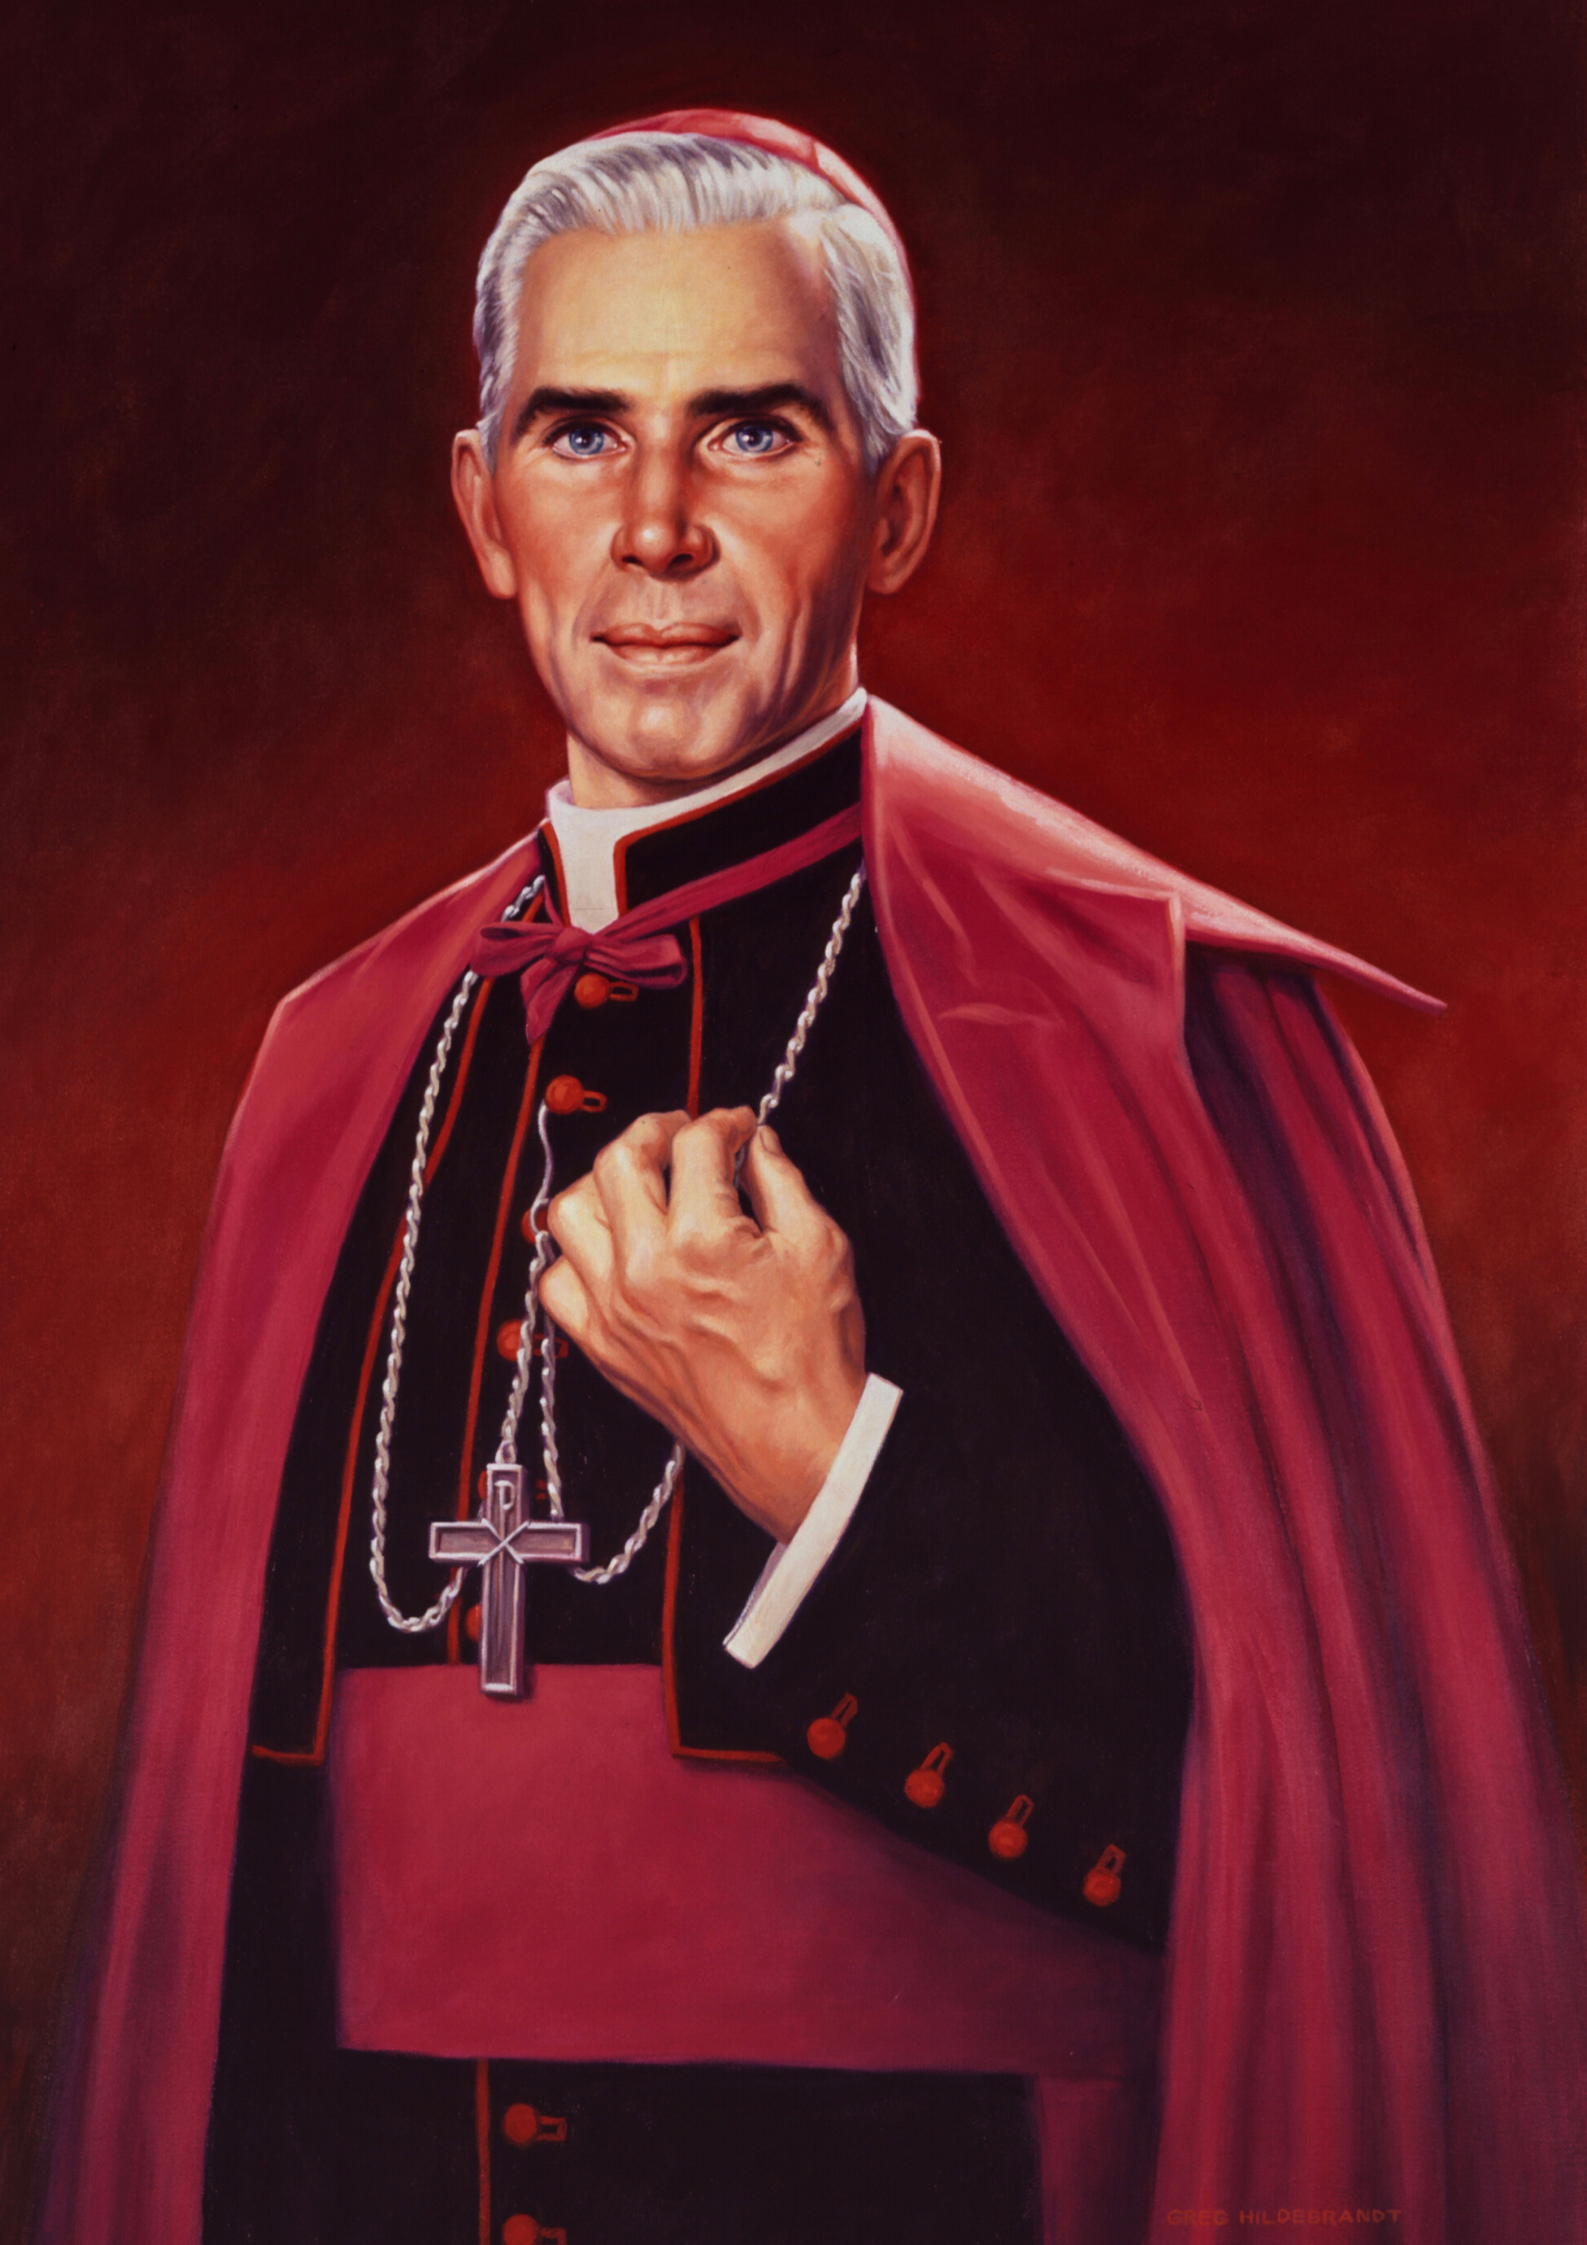
\includegraphics[scale=0.5]{./assets/imagem.jpg} \par
  NOVENA A/À <NOME_SANTO>
}
\author{seu_nome, Nina Freitas}
\date{INICIO_NOVENA/DATA_LITURGICA}


\newcommand*\makecover{
    \usetikzlibrary{positioning}
    \thispagestyle{empty}

    \begin{tikzpicture}[overlay,remember picture]
     \node[] at (0,0) {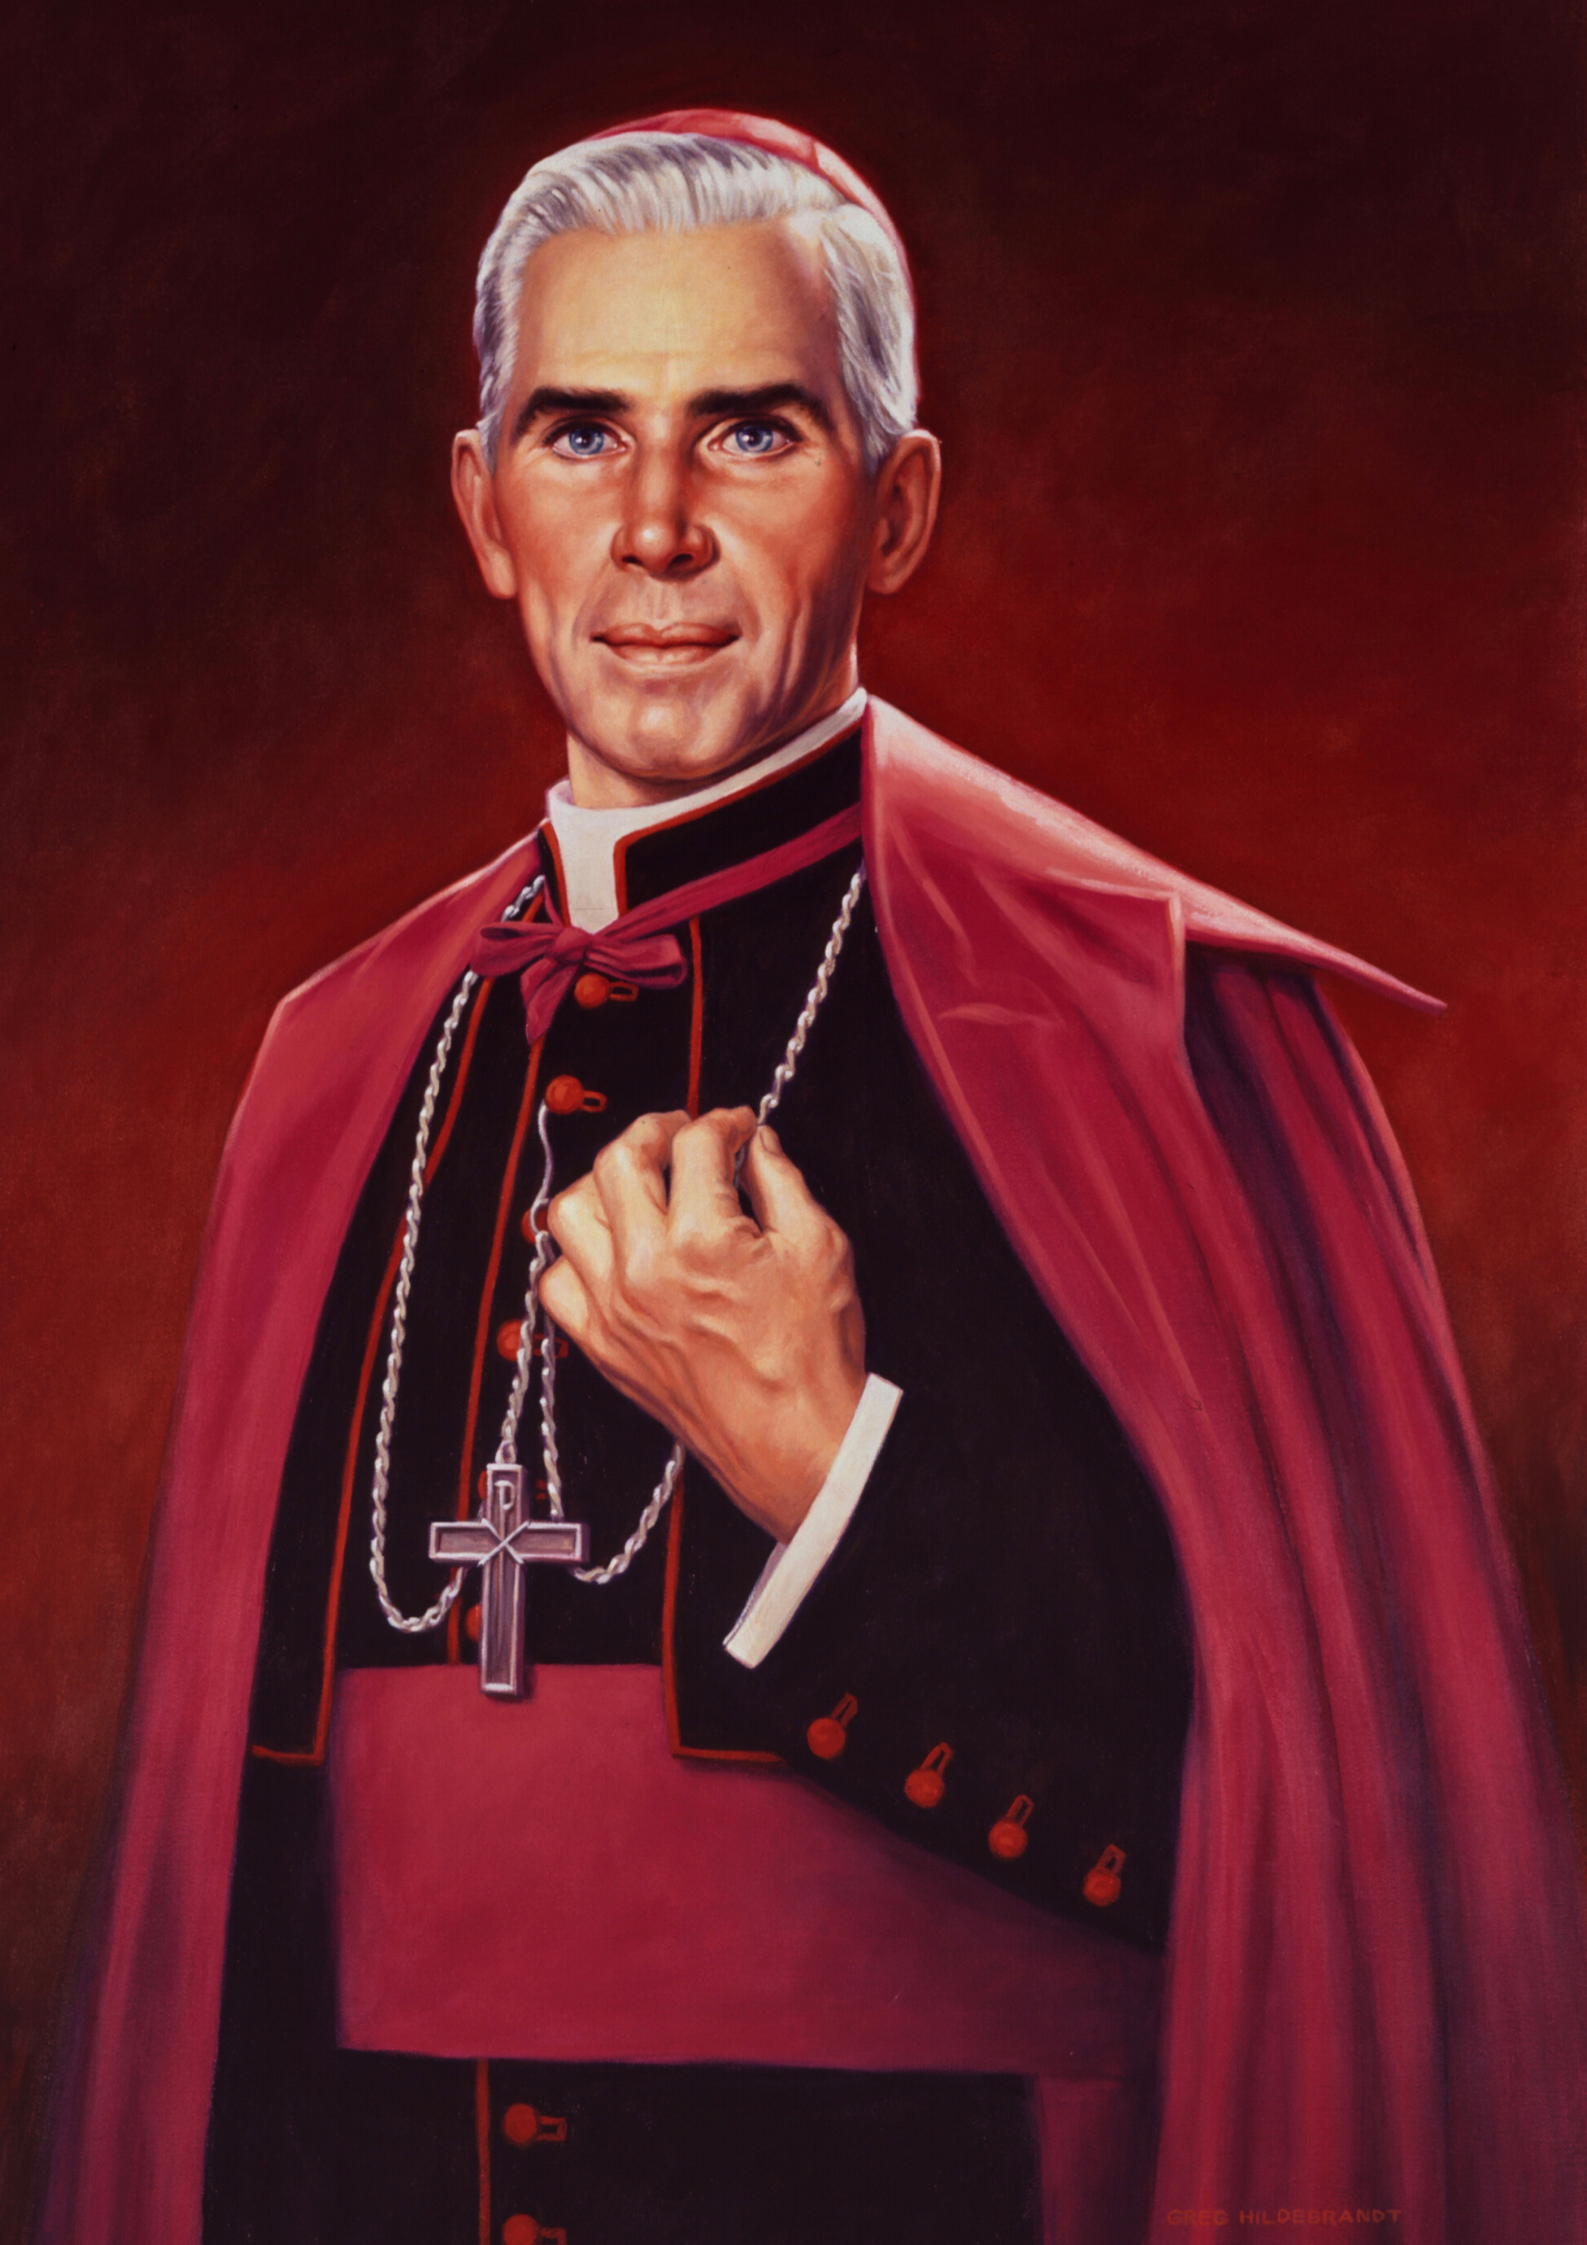
\includegraphics[height=\paperheight]{./assets/imagem.jpg}};
    \end{tikzpicture}
    \newpage
}


\begin{document}


% \maketitle
\makecover



\pagestyle{fancy}
\fancyfoot[LO, CE]{
  \includegraphics[scale=0.2]{./assets/cross.png} SANTO_NOME, Rogai por Nós!
}
  
\tableofcontents

\centering

\section{Orações}\label{oracoes}


\subsection{Oração Inicial}

\subsection{Oração Final}




\section{Dias}
\label{sec:orgb503227}

\subsection{Primeiro Dia}
\label{sec:org623c50b}


\ref{oracoes}


\subsection{Segundo dia}
\label{sec:orgc271256}



\ref{oracoes}

\subsection{Terceiro dia}
\label{sec:orga5ef56a}


\ref{oracoes}



\subsection{Quarto dia}
\label{sec:orgd897ea0}


\ref{oracoes}

\subsection{Quinto dia}
\label{sec:org06f47bb}

\ref{oracoes}

\subsection{Sexto Dia}
\label{sec:org47039c5}

\ref{oracoes}

\subsection{Sétimo dia}
\label{sec:orgb33890d}

\ref{oracoes}

\subsection{Oitavo Dia}
\label{sec:org92a7921}

\ref{oracoes}

\subsection{Nono Dia}
\label{sec:org532001e}

\ref{oracoes}




\textbf{Créditos: }

\end{document}
